% =====================================================================
% Snippet: vector-arrows.tex
% =====================================================================
% USAGE: Vector / gradient visualization on a 2D coordinate system.
% Used in: gradient descent, eigenvectors, force diagrams,
% optimization geometry.
%
% Three variants:
%   A. Single gradient + level sets (gradient descent)
%   B. Multiple eigenvectors from origin
%   C. Tangent + normal at point on curve
%
% Copy whichever fits, replace points/colors.
% =====================================================================

\documentclass[tikz,border=10pt]{standalone}
\usepackage{xcolor,tikz}
\usetikzlibrary{positioning,calc,arrows.meta}

\definecolor{acaBlueLine}{HTML}{3060A8}
\definecolor{acaRedLine}{HTML}{C03030}
\definecolor{acaGreenLine}{HTML}{389050}
\definecolor{acaOrangeLine}{HTML}{D06020}
\definecolor{acaGreyLine}{HTML}{606060}

\tikzset{
  vec arrow/.style={
    -{Stealth[length=5pt 1.2, width'=0pt 0.6]},
    line width=1.0pt,
    shorten >=0pt, shorten <=0pt,
  },
}

\begin{document}
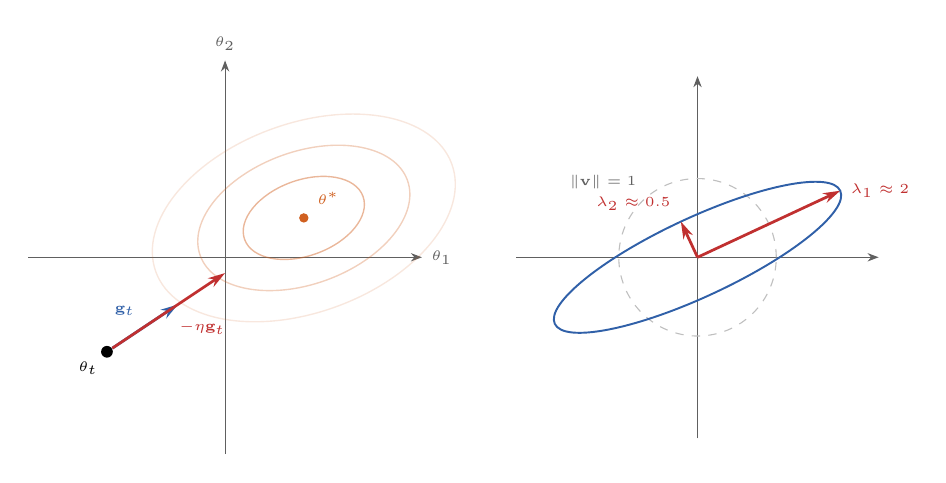
\begin{tikzpicture}

%% COPY-START (Variant A — Gradient descent on level sets) ===========

% Coordinate system
\draw[acaGreyLine, -{Stealth[length=4pt]}] (-2.5, 0) -- (2.5, 0) node[right, font=\tiny] {$\theta_1$};
\draw[acaGreyLine, -{Stealth[length=4pt]}] (0, -2.5) -- (0, 2.5) node[above, font=\tiny] {$\theta_2$};

% Level sets (3 concentric ellipses centered at minimum)
\def\minX{1.0}
\def\minY{0.5}
\foreach \r/\op in {2.0/15, 1.4/30, 0.8/45} {
  \pgfmathsetmacro\ry{\r*0.6}
  \draw[acaOrangeLine, opacity=\op/100, line width=0.5pt, rotate around={20:(\minX, \minY)}]
    (\minX, \minY) ellipse (\r cm and \ry cm);
}
% Minimum point θ*
\node[circle, fill=acaOrangeLine, inner sep=1.2pt] (min) at (\minX, \minY) {};
\node[anchor=south west, font=\tiny, color=acaOrangeLine] at (\minX + 0.05, \minY + 0.05) {$\theta^*$};

% Current point θ_t
\node[circle, fill=black, inner sep=1.5pt] (cur) at (-1.5, -1.2) {};
\node[anchor=north east, font=\tiny] at (-1.5, -1.2) {$\theta_t$};

% Gradient vector (blue): from θ_t, length scaled
\draw[vec arrow, acaBlueLine] (cur) -- ++(0.9, 0.6)
  node[midway, above left, font=\tiny, color=acaBlueLine] {$\mathbf{g}_t$};

% Update direction (red, opposite of gradient, scaled by lr)
\draw[vec arrow, acaRedLine] (cur) -- ++(1.5, 1.0)
  node[midway, below right, font=\tiny, color=acaRedLine] {$-\eta \mathbf{g}_t$};

%% COPY-END Variant A ================================================


%% COPY-START (Variant B — Eigenvectors) =============================

\def\xB{6}
\def\yB{0}

% Coordinate axes
\draw[acaGreyLine, -{Stealth[length=4pt]}] (\xB - 2.3, \yB) -- (\xB + 2.3, \yB);
\draw[acaGreyLine, -{Stealth[length=4pt]}] (\xB, \yB - 2.3) -- (\xB, \yB + 2.3);

% Unit circle (before transform)
\draw[acaGreyLine!40, dashed, line width=0.4pt]
  (\xB, \yB) circle (1);
\node[font=\tiny, color=acaGreyLine] at (\xB - 1.2, \yB + 0.95) {$\|\mathbf{v}\| = 1$};

% Ellipse (after transform, scaled by eigenvalues λ_1=2, λ_2=0.5)
\draw[acaBlueLine, line width=0.7pt, rotate around={25:(\xB, \yB)}]
  (\xB, \yB) ellipse (2 and 0.5);

% Eigenvectors (red, scaled by λ)
% v_1: λ_1 ≈ 2, direction 25°
% Note: PGF macro names cannot have digit-letter sequences (e.g. \v1x
% parses '1x' as "1*x"). Use \vAx / \vBx instead.
\pgfmathsetmacro\vAx{\xB + 2 * cos(25)}
\pgfmathsetmacro\vAy{\yB + 2 * sin(25)}
\draw[vec arrow, acaRedLine] (\xB, \yB) -- (\vAx, \vAy)
  node[right, font=\tiny, color=acaRedLine] {$\lambda_1 \approx 2$};
% v_2: λ_2 ≈ 0.5, direction 115° (perpendicular)
\pgfmathsetmacro\vBx{\xB + 0.5 * cos(115)}
\pgfmathsetmacro\vBy{\yB + 0.5 * sin(115)}
\draw[vec arrow, acaRedLine] (\xB, \yB) -- (\vBx, \vBy)
  node[above left, font=\tiny, color=acaRedLine] {$\lambda_2 \approx 0.5$};

%% COPY-END Variant B ================================================

\end{tikzpicture}
\end{document}
